% Тут используется класс, установленный на сервере Papeeria. На случай, если
% текст понадобится редактировать где-то в другом месте, рядом лежит файл matmex-diploma-custom.cls
% который в момент своего создания был идентичен классу, установленному на сервере.
% Для того, чтобы им воспользоваться, замените matmex-diploma на matmex-diploma-custom
% Если вы работаете исключительно в Papeeria то мы настоятельно рекомендуем пользоваться
% классом matmex-diploma, поскольку он будет автоматически обновляться по мере внесения корректив
%

% По умолчанию используется шрифт 14 размера. Если нужен 12-й шрифт, уберите опцию [14pt]
\documentclass[14pt]{matmex-diploma}
\usepackage{graphicx}                  % Для вставки рисунков
\usepackage{graphics} 
\graphicspath{{images/}{pictures/}}    % можно указать папки с картинками
\usepackage{svg}
\usepackage{amsmath}
\usepackage{listings}
\usepackage{caption}
\usepackage{float}

%\usepackage{fontspec}
%\usepackage{polyglossia}
%\setdefaultlanguage{russian}
%\setmainfont[Ligatures=TeX]{Times New Roman}
%\newfontfamily\cyrillicfont{Times New Roman}

%\usepackage{fontspec}
%\usepackage{polyglossia}
%\setmainlanguage{russian}
%\setotherlanguage{english}

\defaultfontfeatures{Ligatures=TeX, Scale=MatchUppercase}

\DeclareCaptionFont{white}{\color{white}} %% это сделает текст заголовка белым

\begin{document}
% Год, город, название университета и факультета предопределены,
% но можно и поменять.
% Если англоязычная титульная страница не нужна, то ее можно просто удалить.
\filltitle{ru}{
    chair              = {Кафедра системного программирования},
    title              = {Создание Python обёртки над библиотекой линейной разреженной алгебры},
    % Здесь указывается тип работы. Возможные значения:
    %   coursework - Курсовая работа
    %   diploma - Диплом специалиста
    %   master - Диплом магистра
    %   bachelor - Диплом бакалавра
    type               = {coursework},
    position           = {студента},
    group              = 271,
    author             = {Алимов Павел Геннадьевич},
    supervisorPosition = {к.\,ф.-м.\,н., доцент кафедры информатики},
    supervisor         = {Григорьев С.\,В.},
    reviewerPosition   = {ст. преп.},
%    reviewer           = {Привалов А.\,И.},
%    chairHeadPosition  = {д.\,ф.-м.\,н., профессор},
%    chairHead          = {Хунта К.\,Х.},
%   university         = {Санкт-Петербургский Государственный Университет},
%   faculty            = {Математико-механический факультет},
%   city               = {Санкт-Петербург},
%   year               = {2013}
}
\maketitle
\tableofcontents

\lstset{ %
%language=DOT,                 % выбор языка для подсветки (здесь это DOT)
basicstyle=\small\sffamily, % размер и начертание шрифта для подсветки кода
numbers=left,               % где поставить нумерацию строк (слева\справа)
numberstyle=\tiny,           % размер шрифта для номеров строк
stepnumber=1,                   % размер шага между двумя номерами строк
numbersep=5pt,                % как далеко отстоят номера строк от подсвечиваемого кода
backgroundcolor=\color{white}, % цвет фона подсветки - используем \usepackage{color}
showspaces=false,            % показывать или нет пробелы специальными отступами
showstringspaces=false,      % показывать или нет пробелы в строках
showtabs=false,             % показывать или нет табуляцию в строках
frame=tb,              % рисовать рамку вокруг кода
tabsize=2,                 % размер табуляции по умолчанию равен 2 пробелам
captionpos=t,              % позиция заголовка вверху [t] или внизу [b] 
breaklines=true,           % автоматически переносить строки (да\нет)
breakatwhitespace=false, % переносить строки только если есть пробел
escapeinside={\%*}{*)}   % если нужно добавить комментарии в коде
}

%\makeatletter
%\long\def\@makecaption#1#2{%
%  \vspace\abovecaptionskip
%    \bfseries #1: #2
%  \vspace\belowcaptionskip}%
%\makeatother

% У введения нет номера главы
\section*{Введение}


Зачастую решения задач в реальном мире сводятся к решению
систем линейных уравнений, решению дифференциальных уравнениям в частных производных,
вычислению над наборами статистических данных и тому подобным подходам, 
которое удобно производить с помощью компьютера.
И как результат такого перехода возникает необходимость представления объектов 
в форме удобной для проведения вычислений над ними и хранения результатов, 
и в качестве такой формы можно выбрать матрицы.

При этом вышеупомянутые объекты не существуют изолированно друг от друга, 
между ними бывают зависимости или отношения, 
и часто встречается необходимость выявления более сложных взаимосвязей между объектами.
Если эти отношения между объектами представить в виде графа, 
то в терминах теории графов выявления более сложных зависимостей является задачей достижимости.
Одним из способов
задания отношений между объектами графа является описание
ограничений на пути между вершинами. 
Для этого можно использовать контекстно-свободные грамматики над алфавитом меток рёбер графа.

Проблема в том, что существующие для реальных задач графы зачастую являются очень большими
и при представлении в виде матриц оказываются не очень плотными, 
то есть в них много ничего не значащих элементов,
для их описания можно использовать разреженные матрицы. 
Из-за размера графов вычисления над ними занимают много времени, так, к примеру,
в своём исследовании Йохем Куйперс и др. \cite{Kuijpers} провели сравнительный анализ наиболее
известных алгоритмов поиска путей в графе с контекстно-свободными ограничениями и пришли к выводу, что существующие реализации 
обладают большим временем работы.

Но, в то же время, студенты кафедры Системного Программирования 
Никита Мишин и др. показали \cite{evaluation_cfpq_mm}, что использование технологии
GPGPU может ускорить выполнение контекстно-свободных запросов.
При этом при помощи разреженных матриц можно ускорить вычисления и обрабатывать большие матрицы на GPU.
Вкупе с этим существуют различные библиотеки реализаций алгебраических действий над разреженными матрицами
 для вычислений на GPU, такие как \\ 
clSPARSE\footnote{Библиотека работы с разреженными матрицами.
Исходный код библиотеки: https://github.com/clMathLibraries/clSPARSE. Дата посещения: 13.02.2021.},
CuBool\footnote{Библиотека работы с разреженными матрицами.
Исходный код библиотеки: https://github.com/JetBrains-Research/cuBool. Дата посещения: 13.02.2021.}
и прочие, написанные на \textit{C},
и при обосновании выбора библиотеки для использования необходимо иметь результаты сравнения их эффективности.
Вместе с тем уже существует готовый инструментарий\footnote{Окружение для разработки, тестирования и оценки эффективности 
алгоритмов, решающих задачи вычисления запросов в графах с ограничениями на пути между вершинами в виде формальных языков.
Исходный код окружения: https://github.com/JetBrains-Research/CFPQ\_PyAlgo. Дата посещения: 26.12.2020.
},
созданный студентами кафедры Системного Программирования, Арсением Тереховым, Ильёй Эпельбаумом и др.,
для проведения экспериментов над графами с контекстно-свободными ограничениями,
написанный на \textit{Python}.

Таким образом мы приходим к тому, что  
необходимо иметь возможность  в \textit{Python} вызывать функции библиотек, написанных на \textit{C},
взяв за основу интерфейс библиотеки \textit{CuBool},
а значит требуется обёртка над ними, 
позволяющая обращаться к \textit{C} функциям из \textit{Python}.



\section{Цели и задачи}
\textbf{Цель} --- создание обёртки для библиотеки алгебраических действий над разреженными матрицами. 

\textbf{Задачи}:
\begin{enumerate}
    \item Выбрать инструмент для создания обёртки, позволяющей вызывать функции библиотек из $Python$.
    \item Создать обёртку над библиотекой CuBool.
\end{enumerate}

\section{Обзор инструментов для создания обёртки}
Исходя из того, что библиотеки написаны на \textit{C/C++}, а тестовое окружение
для алгоритма решения задачи контестно-свободной достижимости \cite{cfpq_matrix} написано на $Python$,
следует, что выбранный инструмент должен позволять вызывать функции \textit{C/C++} из \textit{Python}. 
А также по возможности хотелось бы не вносить изменения в исходный код библиотек, так как внесённые изменения
могут привести к ухудшению их производительности, приходим к следующим требованиям для инструмента.

\begin{itemize}
    \item Инструмент должен позволять вызывать функции написанные на \textit{C/C++} из $Python$.
    \item Инструмент не должен требовать изменения исходного кода написанного на \textit{C/C++}.
\end{itemize}

Под первый критерий, как самый общий, подходят следующие инструменты: SWIG, CFFI, Boost Python, Ctypes, Python/C API.
Рассмотрим эти инструменты на соответствие второму критерию.

\textbf{SWIG \textit{(Simplified Wrapper and Interface Generator)}}\footnote{
Официальный сайт SWIG: http://www.swig.org.
Дата посещения: 26.12.2020.}
--- это инструмент разработки программного обеспечения,
который связывает программы,
написанные на $C$ и \textit{C++}, с множеством языков программирования высокого уровня,
таких как: \textit{Python, Javascript, Ruby и другие}.

Требования к использованию:
\begin{itemize}
    \item исходный код на \textit{C/C++};
    \item специальный файл интерфейса, написанный на SWIG, для исходного кода;
    \item собранная библиотека исходного кода вместе с файлом интерфейса.
\end{itemize}

Вывод ---  этот инструмент вполне подходит для создания нужной
обёртки, но требует ручной сборки библиотеки, то есть не удовлетворяет второму критерию.

\textbf{CFFI \textit{(C Foreign Function Interface)}}\footnote{
Официальный сайт CFFI: https://cffi.readthedocs.io/en/latest/.
Дата посещения: 26.12.2020.}
--- 
позволяет взаимодействовать практически с любым кодом C из Python на основе C-подобных объявлений.


Требования к использованию:
\begin{itemize}
    \item исходный код только на $C$. Нет поддержки условных директив препроцессора;
    \item собранная библиотека исходного кода.
\end{itemize}

Вывод ---  этот инструмент не поддерживает условные директивы препроцессора, а, к примеру, библиотека \textit{clSPARSE}
написана на \textit{C++} и обёрнута в $C$, и отсюда следует вывод, что \textit{CFFI} не подходит для реализации обёртки.

\textbf{Boost Python}\footnote{
Официальный сайт Boost Python: https://www.boost.org/doc/libs/1\_75\_0/libs/python/doc/html/index.html.
Дата посещения: 26.12.2020.}
--- 
это фреймворк для взаимодействия $Python$ и \textit{C++}.
Он позволяет обращаться к функциям и объектам классов \textit{C++} для $Python$ и наоборот.

Требования к использованию:
\begin{itemize}
    \item исходный код на \textit{C/C++};
    \item написанная обёртка над исходным кодом с использованием функций из фреймворка Boost;
    \item собранная библиотека исходного кода.
\end{itemize}

Вывод ---  этот инструмент требует изменения исходного кода библиотек, для создания обёртки над ней,
то есть не подходит по второму критерию.

\textbf{Ctypes}\footnote{
Официальный сайт ctypes: https://docs.python.org/3/library/ctypes.html.
Дата посещения: 26.12.2020.}
--- 
это библиотека для языка Python, которая предоставляет типы данных, совместимые с C,
и позволяет вызывать функции библиотек написанных на \textit{C} в \textit{Python}.
\textit{Ctypes} можно использовать для обертывания этих библиотек на Python.

Требования к использованию:
\begin{itemize}
    \item исходный код только на \textit{C}. Нет поддержки \textit{C++};
    \item Собранная библиотека исходного кода.
\end{itemize}

Вывод --- этот инструмент
полностью удовлетворяет по функциональности и возможностям, и не
требует никаких дополнительных действий для создания обёртки, то есть подходит по обоим критериям.

\textbf{Python/C API}\footnote{
Официальный сайт Python/C API: https://docs.python.org/3.8/c-api/.
Дата посещения: 26.12.2020.}
--- 
дает программистам на $C$ и \textit{C++} доступ к интерпретатору Python на различных уровнях.
API можно использовать и с \textit{C++}, но для краткости его обычно называют \textit{Python/C API}.

Требования к использованию:
\begin{itemize}
    \item исходный код написанный с использованием библиотеки \textit{"python"} для \textit{C/C++};
    \item Собранный \textit{C/C++} файл в модуль Python.
\end{itemize}

Вывод ---  этот инструмент требует исходного кода
написанного с использованием библиотеки $python$, 
а, выбранная библиотека CuBool не соответствует этому требованию,
то есть использование этого интсрумента требует внесения
изменений в исходную библиотеку, то есть не подходит по второму критерию.

Таким образом можно сделать заключение, что из вышеперечисленных инструментов подходит только \textit{Ctypes},
так как остальные инструменты не удовлетворяют как минимум одному из поставленных критериев.

\section{Реализация}
Архитектуру всего проекта можно описать следующим образом. 
На вход реализованному с помощью вышеупомянутого окружения \\ \textit{CFPQ\_PyAlgo}\footnote{
Окружение для разработки, тестирования и оценки эффективности 
алгоритмов, решающих задачи вычисления запросов в графах с ограничениями на пути между вершинами в виде формальных языков.
Исходный код окружения: https://github.com/JetBrains-Research/CFPQ\_PyAlgo. Дата посещения: 26.12.2020.
} алгоритму
подаётся граф и контекстно-свободная грамматика.
А затем выполняется сам алгоритм, используя функции библиотеки разреженной алгербы с помощью созданной в ходе этой работы обёртки, в данном случае CuBool.
На рисунке \ref{pic:projectArch} изображена общая архитектура проекта описанная выше.


\begin{figure}[h]
    \centering
    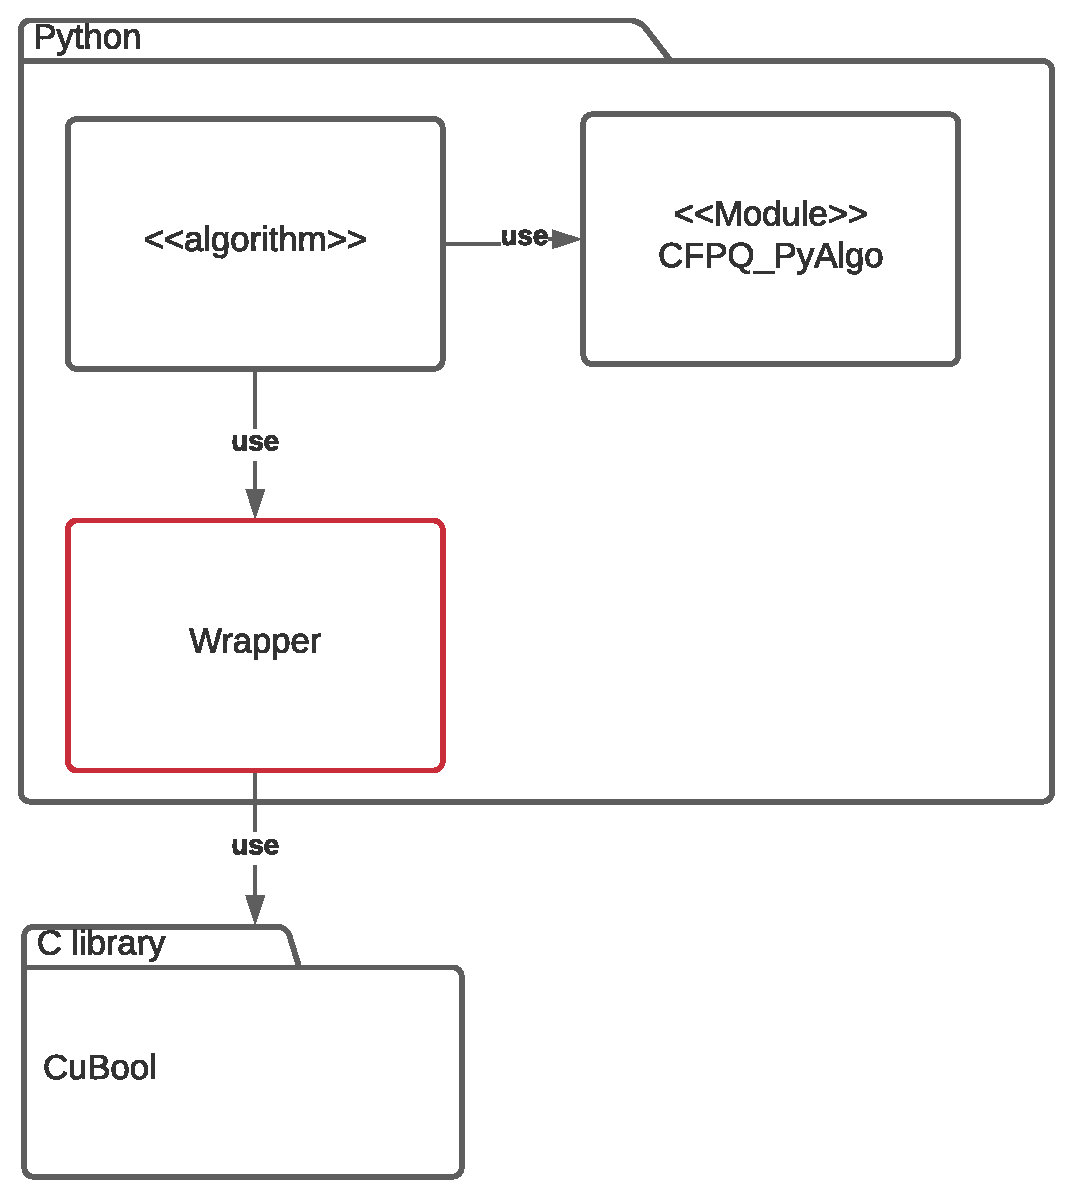
\includegraphics[height=12cm]{pictures/arch.eps}
    \caption{Общая архитектура. Красным выделена цель данной работы.}\label{pic:projectArch}
\end{figure}

\subsection{Обёртка}
Было принято решение делать обёртку, опираясь на API библиотеки CuBool\footnote{
Библиотека работы с разреженными матрицами.
Исходный код библиотеки: https://github.com/JetBrains-Research/cuBool. Дата посещения: 13.02.2021.
}, так как общий интерфейс библиотек должен быть похожим на интерфейс библиотеки CuBool. 
Таким образом была написана обёртка над библиотекой CuBool,
позволяющая выполнять алгебраические операции над матрицами.
При разработке было решено сделать API обёртки похожим на pygraphblas\footnote{
pygraphblas - \textit{Python} обёртка над GraphBLAS API. 
Исходный код обёртки - https://github.com/Graphegon/pygraphblas. Дата посещения: 30.03.2021
},
как на уже существующий известный инструмент работы с матрицами, для упрощения восприятия.

На рисунке \ref{pic:projectPython} представлена получившаяся архитектура решения. 
В ходе работы, в репозитории библиотеки \textit{CuBool}\cite{cuBool} в разделе \textit{python}
был написан модуль \textit{bridge}, в котором определяются функции исходной библиотеки \textit{CuBool},
такие как создание и удаление объекта типа \textit{"матрица"}, поэлементное сложение матриц, произведение Кронекера,
матричное умножение, взятие подматрицы, создание копии, транспонирование, получение информации о матрице. 
А также написан модуль \textit{wrapper},
который хранит определения уже упомянутых функций в виде единого объекта и предоставляет доступ к ним.
При этом был создан класс \textit{Matrix}, который предоставляет доступ пользователю к библиотечным функциям с помощью своих методов.
Для упрощения ввода и вывода матриц и демонстрации результата были написаны функции,
позволяющие генерировать матрицу, считывать матрицу в mtx формате из файла и записывать матрицу в файл в mtx формате.
Функция генерации матриц в качестве входных параметров принимает плотность заполнения и кортеж из числа столбцов и строк,
и возвращает случайным образом заполненную матрицу заданной формы и плотности. 

\begin{figure}[h!]
    \centering
    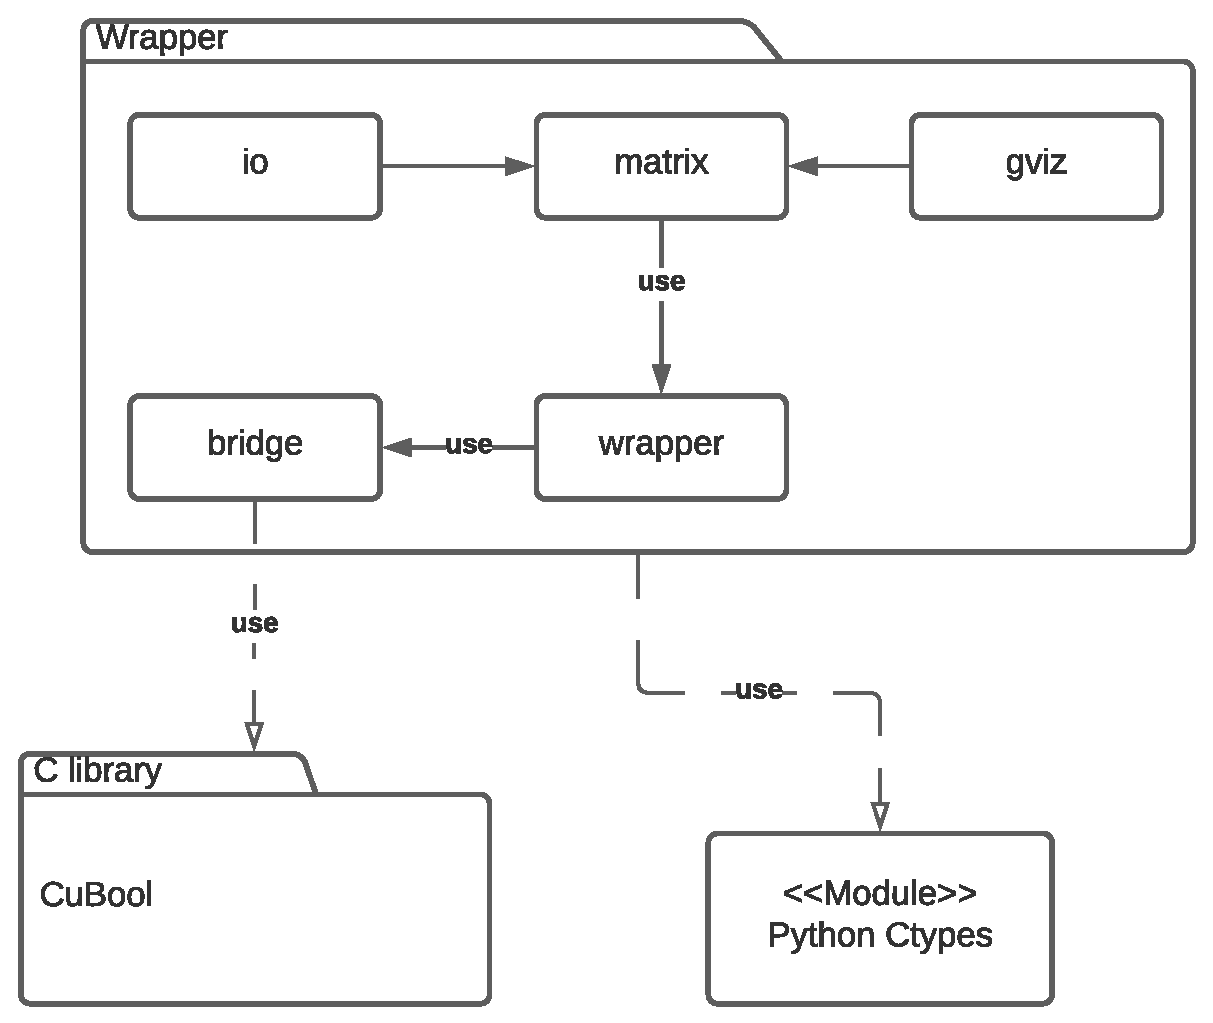
\includegraphics[height=13.5cm]{pictures/pycubool.eps}
    \caption{Архитектура работы.}\label{pic:projectPython}
\end{figure}
\newpage

\subsection{Регрессионные тесты}
С помощью вышеописанных функций был сгенерирован набор матриц различной формы для тестирования 
каждой из матричных операций.

Заодно были написаны сами тесты на каждую матричную операцию, которые 
считывают уже сгенерированную матрицу из входного файла,
применяют к входной матрице соответствующую функцию и сравнивают получившийся результат с прошлым результатом работы.

\subsection{Графовое представление матрицы смежности}
Также была написана функция, переводящая матрицы в \textit{Graphviz} скрипт\footnote{
Graphviz - это программа для визуализации графов.
Официальный сайт - https://graphviz.org. Дата посещения: 30.03.2021.
},
для возможности визуализации представляемых графов.
Было принято решение добавить возможность выбора цвета для ребёр и вершин графов,
а также номер начальной вершины и метки на рёбрах для построения соответствующей строки на языке \textit{DOT},
который поддерживает \textit{Graphviz}.
Таким образом получилась функция, которые по нескольким входным матрицам строит их графовое представление в рамках одного графа,
что можно использовать, в частности, для визуализации графов с контекстно-свободными ограничениями.

К примеру, для двух матриц смежности:
$$a = 
\begin{pmatrix}
  0& 0& 1& 0& 0& 0& 0\\
  0& 0& 1& 0& 0& 0& 0\\
  0& 0& 0& 0& 0& 0& 1\\
  0& 0& 0& 0& 0& 1& 0\\
  0& 0& 0& 0& 0& 1& 0\\
  0& 0& 0& 0& 0& 0& 1\\
  0& 0& 0& 0& 0& 0& 0
\end{pmatrix} \text{ и }
b = 
\begin{pmatrix}
  0& 0& 0& 0& 0& 0& 0\\
  0& 0& 0& 0& 0& 0& 0\\
  1& 1& 0& 0& 0& 0& 0\\
  0& 0& 0& 0& 0& 0& 0\\
  0& 0& 0& 0& 0& 0& 0\\
  0& 0& 0& 1& 1& 0& 0\\
  0& 0& 1& 0& 0& 1& 0
\end{pmatrix}\text{;}
$$
задав для матрицы \textit{a} красный цвет рёбер и для матрицы \textit{b} зелёный цвет рёбер,
получим скрипт описанный в листинге \ref{lst:dotScript}, по которому строится граф представленный на рисунке \ref{pic:graph}.

\newpage
\begin{lstlisting}[caption={Скрипт на языке DOT, описывающий граф.}, label=lst:dotScript]
digraph G {
    graph [label=Test];
    node [color=black];
    1 -> 3 [label=a,color=red];
    2 -> 3 [label=a,color=red];
    3 -> 7 [label=a,color=red];
    4 -> 6 [label=a,color=red];
    5 -> 6 [label=a,color=red];
    6 -> 7 [label=a,color=red];
    3 -> 1 [label=b,color=green];
    3 -> 2 [label=b,color=green];
    7 -> 3 [label=b,color=green];
    6 -> 4 [label=b,color=green];
    6 -> 5 [label=b,color=green];
    7 -> 6 [label=b,color=green];
}
\end{lstlisting}

\begin{figure}[hb]
    \centering
    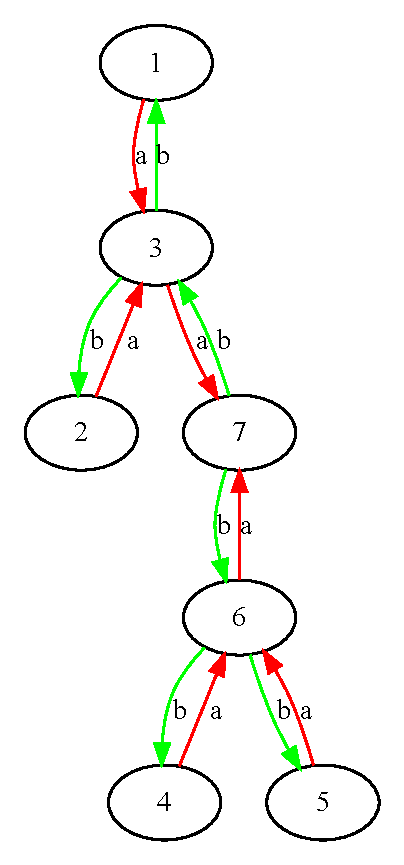
\includegraphics[height=12cm]{pictures/graphviz.eps}
    \caption{Граф с метками на рёбрах}\label{pic:graph}
\end{figure}

\subsection{Примеры использования}
В дополнение к созданной обёртке были написаны примеры\footnote{
Примеры использования методов класса Matrix.
Исходный код примеров: https://github.com/JetBrains-Research/cuBool/tree/master/python/examples. Дата посещения: 04.06.2021.
}
использования методов класса \textit{Matrix}
с выводом полученного результата и подробными комментариями. 
А также создан сопровождающий текстовый документ\footnote{
Документ со текстом всех примеров использования методов класса Matrix и результатом их исполнения.
Ссылка на документ: https://github.com/JetBrains-Research/cuBool/blob/master/docs/examples/python\_examples.md.
Дата посещения: 04.06.2021.}
с кодом примеров и соответствующими результатами их исполнения.



\section*{Заключение}
В рамках данной работы были получены следующие результаты:
\begin{itemize}
    \item был выбран инструмент \textit{Ctypes} для создания обёртки;
    \item с помощью выбранного инструмента в репозитории библиотеки \textit{CuBool}\cite{cuBool}
          на \textit{Python} реализовано:
        \begin{enumerate}
            \item чтение матрицы из файла;
            \item запись матрицы в файл;
            \item создание матрицы, как объекта библиотеки;
            \item вызов библиотечных алгебраических операций над матрицами;
            \item написаны регрессионные тесты к обёртке;
            \item перевод матрицы в \textit{Graphviz} скрипт;
            \item написаны примеры использования.
        \end{enumerate}
\end{itemize}   

\bibliographystyle{ugost2008ls}
\bibliography{diploma.bib}
\end{document}